\section{Aktuelle Bewertung der Kraftwerksreserven zur Netzstabilisierung und Reserveleistungsvorhaltung}

	Im vorherigen Kapitel wurden die verschiedene Reserven in Deutschland beleuchtet und definiert. 
	Außerdem fand eine erste Bewertung der aktuellen Situation statt. Im Folgenden sollen nun die technische und logistische Realisierbarkeit bzw. Nutzbarkeit der verschiedenen Reserven aufgezeigt werden. 
	Außerdem soll ein Ausblick auf zukünftige Entwicklungen, Möglichkeiten und Gefahren gegeben werden. 
	Dabei spielt auch der russische Überfall auf die Ukraine ausschlaggebende eine Rolle. 
	Dieser wird in einer Aufnahme der momentanen deutschen Strategie zur Versorgungssicherheit im Winter berücksichtigt.

	\subsection{Bewertung der logistischen Situation der Reserven}
	
		Die Erhebung der Daten im Punkt Logistik gestaltet sich als herausfordernd, da die logistische Situation von unabhängige Stelle nicht überwacht wird. 
		Es können sich lediglich Aussagen von den Kraftwerksbetreibern selbst eingeholt werden.
	
		\subsubsection{Logistischer Stand der Braunkohle} \label{sect: Braunkohle}
		
			In der Sicherheitsbereitschaft befinden sich in Deutschland ausschließlich Braunkohlekraftwerke, welche durch zwei Energieversorgungsunternehmen betrieben werden.
			Zum einen die RWE Power AG mit den zwei Blöcken Niederaußem E und F in Bergheim und dem Block Neurath C in Grevenbroich (Rheinischen Braunkohlerevier).
			Zum anderen die Lausitzer Energie und Kraftwerke AG, im Folgenden LEAG, mit den zwei Blöcken Jänschwalde E und F in Teichland (Lausitzer Braunkohlerevier) \cite{Excel_Kraftwerksliste}. \\
	
			Die Blöcke des Kraftwerks Jänschwalde werden durch Tagebaue der LEAG in Jänschwalde, Welzow-Süd, Nochten und Reichwalde versorgt. 
			Der Transport wird auf der Schiene durch einen firmeneigenen Eisenbahnbetrieb realisiert. 
			Der Abbau des Tagebaus Jänschwalde stoppt voraussichtlich im Jahr 2023, da dieser dann erschöpft ist. 
			Die Versorgung wird anschließend von den übrigen drei Abbaustandorten übernommen.
			Das Kraftwerk Jänschwalde stellt mit sechs Kraftwerksblöcken ein Großkraftwerk dar.
			Da die Kraftwerksblöcke aus der Sicherheitsbereitschaft wieder aktiv am Strommarkt teilnehmen, lässt sich Personalproblem ausschließen \cite{LEAG_Braunkohleversorgung}. \\
			
			Die in Sicherheitsbereitschaft befindlichen Blöcke Niederaußem E und F sowie Neurath C werden ebenfalls durch RWE-eigene Tagebaue versorgt. 
			Hierbei handelt es sich um die Förderstätten Garzweiler, Hambach und Inden. 
			Der Transport erfolgt über eine Eisenbahngesellschaft der RWE. 
			Auch bei diesen drei Blöcken handelt es sich um Teile von größeren Kraftwerkskomplexen. 
			Auch die Kraftwerksblöcke der RWE Power AG nehmen wieder aktiv am Strommarkt teil, wodurch sich die Personalsituation als unkritisch erweist \cite{Mail_RWE}. 
	
		\subsubsection{Logistischer Stand der Steinkohle} \label{sect: Steinkohle}
		
			Die deutschen Steinkohlekraftwerke, welche nicht mehr aktiv am Markt teilnehmen und noch nicht endgültig stillgelegt sind, befinden sich in der Netzreserve. 
			Diese ist im KVGB und $\S$ 13b des EnWG rechtlich geregelt. 
			Bei den Betreibern handelt es sich um die EnBW Energie Baden-Würtemberg AG, STEAG, Uniper Kraftwerke GmbH, Kraftwerk Mehrum GmbH und das Großkraftwerk Mannheim \cite{Excel_Kraftwerksliste}. \\
			
			Die logistische Situation ist weiterhin angespannt. 
			Niedrige Pegelstände von Rhein und Neckar, sowie der fehlende Gleisausbau in Deutschland erschwerten den Steinkohletransport erheblich. 
			Die RAG Deutsche Steinkohle AG war der alleinige Betreiber deutscher Steinkohlebergwerke. 
			Diese stellte den Abbau 2018 komplett ein, da dieser nicht mehr wirtschaftlich war.
			Dadurch sind die Betreiber zu \SI{100}{\percent} auf Importe angewiesen \cite{Ende_Steinkohle}. \\
			
			Die EnBW verstärkt seit Juli 2022 ihre Bemühungen zur Beschaffung und Erschließung von Flächen zur zusätzlichen Lagerung von Steinkohle.
			Die Personalsituation ist ebenfalls angespannt, da diese langfristig mit der Prämisse der Stilllegung geplant war. 
			Die fünf Blöcke der Netzreserve werden jedoch aller Voraussicht nach nicht wieder am Markt teilnehmen, da diese nach Aussage der EnBW aus technischen Gründen nicht ununterbrochen zur Stromerzeugung eingesetzt werden können. 
			Grund hierfür ist das fortgeschrittene Alter der Anlagen \cite{EnBW_Steinkohle}. \\
			
			Der Stromerzeuger STEAG betreibt zwei Kraftwerke in der Netzreserve (Boxberg und Weiher 3 im Saarland). 
			Die herausfordernde Lage der Kohleversorgung, auch mit Hinblick auf den kommenden Winter, veranlasste das Wirtschaftsministerium des Saarlandes zu einem Logistik-Gipfel. 
			Zu den Teilnehmenden gehörten unter anderem der Staatssekretär des Bundesministeriums für Digitales und Verkehr, die STEAG selbst und die DB Cargo. 
			Die Gespräche ergaben eine vorrangige Behandlung von Kohletransporten auf der Schiene gegenüber dem öffentlichen Personennahverkehr, im Falle von Versorgungsengpässen \cite{Logistikgipfel_Saarland}. 
			Dies stellt die Belieferung der Kraftwerke mit Brennstoff sicher. 
			Zusätzlich tritt das Kraftwerk Boxberg zum 28.10.2022 wieder in den Markt ein. 
			Das Schwesterkraftwerk Weiher 3 folgt am 31.10.2022. 
			Ermöglicht wird dies durch das EKBG welches eine Rückkehr in den Strommarkt bis Frühjahr 2024 gestattet \cite{STEAG_Steinkohle}. 
	
	
		\subsubsection{Logistischer Stand des Erdgases}
		
			Infolge des russischen Überfalls auf die Ukraine sanken die deutschen Erdgasimporte aus Russland im September nach Stand vom 03.11.2022 auf null. 
			Zum 03.05.2022 startete die Bundesnetzagentur eine Datenerhebung, um den deutschen Gasverbrauch zu ermitteln \cite{Datenerhebung_Gas}. 
			In einer Pressemitteilung vom 29.09.2022 wurde von einer notwendigen Einsparung in Höhe von \SI{20}{\percent} gesprochen, um die Versorgungssicherheit im Winter zu gewährleisten.
			Das Impulspapier von Acatech spricht sogar von 20 bis \SI{30}{\percent} \cite{Impuls_Acatech_Einsparung}. \\
			
			Deutsche Erdgaskraftwerke, welche nicht mehr im Betrieb sind, befinden sich sowohl in der Netz- als auch in der Kapazitätsreserve. 
			Die Versorgung ist sehr stark von den Netzbetreibern abhängig und die Situation nur sehr schwer vorhersehbar. 
			Deutschlands Gasspeicher sind nach Stand vom 13.12.2022 zu knapp \SI{100}{\percent} gefüllt \textbf{!!QUELLE!!}. 
			Des Weiteren sollen zum Jahreswechsel 22/23 zwei FSRU's in Betrieb genommen werden \cite{LNG_FSRU}.
			Ein zusätzliches Problem bei der Versorgung stellt die Ausrichtung der in Europa vorhandenen Gas-Infrastruktur dar. 
			Diese ist auf einen Gastransport von Ost nach West ausgerichtet. 
			Der Großteil der europäischen LNG-Terminals befindet sich in Westeuropa. 
			Damit ist eine Umkehrung des Gasflusses notwendig. 
			Dieser sogenannte Reverse-Flow wird ermöglicht, indem die Verdichterstationen umgebaut werden. 
			Danach ist ein Gastransport in beide Richtungen bei voller Kapazität möglich \cite{Impuls_Acatech_Reverse_Flow}. \\
			
			Ein eventuelles Verbot der Verstromung von Gas ist im Notfallplan Gas beschrieben.
			Dieser ist in drei Teile unterteilt. 
			Die Frühwarnstufe und die Alarmstufe lassen einen Eingriff des Gesetzgebers vorerst nicht zu. 
			Stattdessen wird auf marktbasierte Maßnahmen zur Regulierung der verbrauchten Gasmengen gesetzt. 			
			Sollte die Notfallstufe Gas ausgerufen werden, wird das Bundesministerium für Wirtschaft und Klima in Zusammenarbeit mit der Bundesnetzagentur als Lastverteiler eingesetzt.
			Zudem kann die Substitution von Erdgas durch andere Brennstoffe angeordnet werden.
			Dieses ist jedoch nur eine von verschiedenen möglichen Maßnahmen, die ergriffen werden können. 
			Da sich Deutschland noch nie in einer derartigen Situation befunden hat, ist nur schwer vorherzusehen von welchen Steuermechanismen Gebrauch gemacht wird \cite{Notfallplan_Gas}.
	
		\subsubsection{Logistischer Stand des Mineralöls}
		
			Durch politisch motivierte Verknappung der Öllieferungen wurde der Preis künstlich angehoben, bis es schließlich 1973 zur ersten Ölknappheit in der Geschichte der Bundesrepublik Deutschland kam.
			Daraufhin wurde 1974 die Internationale Energieagentur gegründet, welche eine zuverlässige Energieversorgung koordinieren soll. 
			Diese empfahl die Einrichtung einer strategischen Ölreserve, zur Absicherung gegen eventuell auftretende Lieferausfälle. 
			Seitdem lagert Deutschland genug Öl, um den Gebäude-, Industrie-, Verkehrs- und Energiesektor für 90 Tage mit Öl zu versorgen \cite{strat_Ölreserve_Geschichte}. \\
			
			In Deutschland gibt es sechs Blöcke in drei Kraftwerken, die sich in der Netzreserve befinden und mit Öl befeuert werden \cite{Excel_Kraftwerksliste}. 
			Die Versorgung erfolgt über Pipelines und Öltanker.
			Die Kraftwerke Ingolstadt in Großmehring und Irsching werden durch die TAL-Pipeline, welche von Triest kommend den großteil Süddeutschlands mit Mineralöl versorgt. 
			Das Kraftwerk Marbach, betrieben durch die EnBW, liegt ebenfalls im Süden Deutschlands und wird durch die Pipeline TAL versorgt. 
			Bei Lieferausfällen besteht in beiden Fällen die Möglichkeit über die nahe gelegene Donau bzw. den Neckar versorgt zu werden, sofern diese genug Wasser führen und Schiffsverkehr zulassen. 
			Sollte auch dieser Versorgungsweg ausfallen, so steht noch die strategische Ölreserve zur Verfügung. 
			Diese garantiert eine Versorgung mit Mineralöl über mindestens 90 Tage und fällt in Realität sogar größer aus (s. Abbildung \ref{Abb. Strategische Ölreserve}).
	
			\begin{figure}[H]
				\centering
				\includegraphics[page=1, width=0.6\textwidth]{./anhang/Ölreserve.png}
				\caption{Vergleich von Ölreserven verschiedener europäischer Länder \cite{IEA_Ölreserven}}
				\label{Abb. Strategische Ölreserve} 
			\end{figure}
		
		
	\subsection{Kapazitätssituation für den Winter 2022/23}
	
		Im ersten Halbjahr 2022 erzeugte Erdgas \SI{30,7}{\tera\watt\hour} elektrischen Strom in Deutschland. 
		Dies entspricht einem Anteil von \SI{11,7}{\percent} an der Gesamterzeugung \cite{Stromproduktion_Erdgas}. 
		Im Hinblick auf drohende Versorgungsengpässe werden die bis dato getroffenen Gegenmaßnahmen beleuchtet. 
	
		\subsubsection{Der zweite Stresstest für die Stromversorgung}
		
			Im Rahmen des vom BMWK in Auftrag gegebenen Stresstests, sollen die Übertragungsnetzbetreiber verschiedene Szenarien für die Versorgungssicherheit im Winter 2022/23 analysieren. 
			Dabei wurde die Gasversorgung, Steinkohleversorgung und eventuell ausfallende Kapazitäten im Ausland in Augenschein genommen.		
			Ein zentraler Punkt der Analyse ist die Annahme, dass Polen keinen Strom exportieren kann, da die Versorgung mit Steinkohle durch Lieferengpässe nicht möglich ist.
			Des Weiteren wurde davon ausgegangen, dass Frankreich bis zum Winter nicht alle Kernkraftwerke an den Markt bringen kann. 
			Diese sind auf Grund von zu hohen Temperaturen, Niedrigwasser, Wartungsarbeiten und Defekten im Sommer teilweise abgeschaltet worden \cite{AKW_Frankreich}. 
			Außerdem geht die Studie im kritischsten der drei Szenarien davon aus, dass Süddeutschland und Österreich die vertraglich geregelte Redispatchleistung aus Gaskraftwerken nicht liefern können. \\
			
			Die Analyse zeigt, dass in den beiden kritischsten Situationen in Deutschland einige Stunden der Lastunterdeckung auftreten können. 
			Des Weiteren wird gezeigt, dass die deutsche Redispatchleistung in keinem der drei Szenarien ausreicht. 
			Die Differenz muss über ausländische Kraftwerke ausgeglichen werden. 
			Der Streckbetrieb der deutschen Kernkraftwerke entspannt die Situation dahingehend, dass Lastunterdeckungen weitestgehend vermieden werden können und der Bedarf an Redispatch ebenfalls sinkt \cite{Stresstest}. \\
			
			Die Empfehlungen der Übertragungsnetzbetreiber lassen sich zu fünf Säulen zusammenfassen, welche die angespannte Versorgungssituation entspannen sollen.
			\begin{itemize}
				\item Transportkapazitäten erhöhen
				\item Redispatch-Potential im Ausland fokussieren
				\item vertragliches Lastmanagement
				\item Reserven nutzbar machen
				\item Nutzung weiterer Kraftwerkskapazitäten absichern
			\end{itemize}
		
		\subsubsection{Umsetzung der Empfehlungen} \label{sect: Atomausstieg}
			
			Am 07.10.2022 wurde vom Bundesrat die Novelle zum Energiesicherheitsgesetz 3.0 verabschiedet. 
			Dieses baut auf verschiedene Säulen zur Anhebung der Kapazitäten für die Stromerzeugung \cite{EnSiG}. 
			\begin{itemize}
				\item Erhöhung der Stromproduktion aus Photovoltaikanlagen
				\item Anreize für die Verstromung von Biogas
				\item Erhöhung der Produktion von Windstrom
				\item Maßnahmen zur Beschleunigung des Netzausbaus
				\item Maßnahmen im LNG-Beschleunigungsgesetz
				\item Erleichterung für den Brennstoffwechsel
				\item Änderungen im Baugesetzbuch
			\end{itemize}
			
			Zur Erhöhung der Produktionskapazitäten wurde außerdem ein Streckbetrieb für 3 verbleibende deutsche Atomkraftwerke beschlossen. 
			Die Meiler Isar 2, Neckar-Westheim 2 und Emsland werden bis maximal Mitte April 2023 am Netz bleiben. 
			Diese sollen die Gaskraftwerke zusätzlich entlasten und Netzengpässe abfedern \cite{Laufzeitverlängerung}. 
			Wie in Abschnitt \ref{sect: Steinkohle} beschrieben, wurden die Versorgungsengpässe bei der Steinkohle überwunden. 
			Zudem sind einzelne Reservekraftwerke ab Oktober wieder in den Markt eingetreten.
			Insgesamt nehmen Steinkohlekraftwerke mit einer Nettoleistung von insgesamt \SI{2,25}{\giga \watt} wieder am Strommarkt teil.
			Auch die Braunkohlekraftwerke aus der Sicherheitsbereitschaft (siehe \ref{sect: Braunkohle}) nehmen inzwischen wieder aktiv am Markt teil.
			Die Blöcke Niederaußem E, F und Neurath C zum 01.10.2022, Jänschwalde E zum 06.10.2022 und Jänschwalde F zum 15.10.2022. 
			Diese summieren sich zu einer Nettoleistung von \SI{1,886}{\giga \watt} auf \cite{Wiedereintritt_Kraftwerke}. 
		
		
\section{Die zukünftige Entwicklung von Kraftwerksreserven}
		
	Der menschengemachte Klimawandel stellt eine gigantische Bedrohung für das Leben auf der Erde dar. 
	Die Energiewende und mit ihr die essenzielle Veränderung des Strom-, Wärme und Verkehrssektors stellen Deutschland vor drastische Herausforderungen. 
	Zur Erreichung des 1,5 Grad Ziels müssen die Emissionen weltweit bilanziell auf null reduziert werden.
	Ohne Reduzierung der \COO-Emissionen (in Deutschland) ist das \COO-Budget zur Einhaltung des 1,5 Grad Ziels in 6 Jahren und 8 Monaten erschöpft (Stand November 2022). !!!\textbf{Frage weltweit oder Deutschland??}!!!.
	Das \COO-Budget für das 2 Grad Ziel hingegen in 24 Jahren und 5 Monaten. 
	Diese Zeiträume zeigen, die Notwendig- sowie Dringlichkeit des Handelns \cite{CO2_Uhr}. \\ 
	
	Dem Stromsektor kommt dabei eine gesonderte Bedeutung zu. 
	Nicht nur bietet dieser den Grundstein für die Dekarbonisierung der übrigen Sektoren, sondern stellt auch heute den größten \COO-Emittenten dar \cite{Umweltbundesamt_Emissionen}. 
	Deshalb ist es wichtig fossile Energieträger sukzessive zu substituieren. 
	Mit der Verankerung des Klimaschutzes zur Generationen- und Freiheitssicherung im Grundgesetz sind die jetzige, aber auch künftige Regierungen verpflichtet, die \COO-Emissionen zu senken und schlussendlich klimaneutral zu werden. 
	Dafür stellte die Ampel-Koalition im November 2021 ihren Koalitionsvertrag vor, der folgende Maßnahmen enthält\cite{Koalitionsvertrag}:
	\begin{itemize}
		\item Atomausstieg bis Ende 2022
		\item Kohleausstieg im Optimalfall bis 2030
		\item Errichtung moderner \Htwo-ready Gaskraftwerke
		\item Zulassung von 15 Millionen vollelektrischen PKW bis 2030
		\item Deckung von \SI{80}{\percent} des Bruttostrombedarfs aus erneuerbaren Energien bis 2030
		\item PV-Ausbau verpflichtend bei gewerblichen Neubauten
		\item PV-Ausbau auf \SI{200}{\giga\watt}
		\item Ausweisung von \SI{2}{\percent} der Landesfläche für Windkraft
		\item Kapazitätserhöhung von Off-Shore Winkraft auf mindestens \SI{30}{\giga\watt} bis 2030, \SI{40}{\giga\watt} bis 2035 und \SI{70}{\giga\watt} bis 2045
		\item Elektrolysekapazität von \SI{10}{\giga\watt} bis 2030
	\end{itemize}
	Bereits im Oktober 2022 verständigte sich die Regierung mit der RWE Generation SE und dem Wirtschaftsministerium Nordrhein-Westfalen auf einen vorzeitigen Braunkohleausstieg im Rheinischen Revier für 2030 \cite{Kohleausstieg_RWE}. \\
	
	In den folgenden Abschnitten werden mit Hilfe von zwei Studien mögliche Energieversorgungsstrukturen für die Jahre 2030 und 2045 aufgezeigt.
	Anhand dieser wird die zukünftige Entwicklung der Kraftwerksreserven analysiert.
	Für das Szenario 2030 wird die Studie "`Klimaneutrales Stromsystem 2035"' der Agora Energiewende genutzt.
	Für das Jahr 2045 wird die Studie "`Energiewende im Sozialen Raum"', welche auf Annahmen des "`Ariadne Report"' des PIK fußt und aus einer Zusammenarbeit von Germanwatch, Global Climate Forum und dem Frauenhofer Institut für Energiewirtschaft und Energiesystemtechnik stammt, genutzt.
%	\textsl{Um jetzige Zustände und künftige Entwicklungen bewerten zu können, bieten Studien und Modelle die Möglichkeit die Energieversorgung der nächsten Generation zu skizzieren. 
%	In den folgenden Abschnitten werden im besonderen Maße die Studien "`Klimaneutrales Stromsystem 2035"' von Agora Energiewende, sowie die Studie "`Energiewende im Sozialen Raum"', einer Zusammenarbeit von Germanwatch, Global Climate Forum und dem Frauenhofer Institut für Energiewirtschaft und Energiesystemtechnik, welche auf Annahmen des "`Ariadne Report"' des Potsdam-Institut für Klimafolgenforschung (PIK) fußt, in Augenschein genommen.}

	\subsection{Aktueller Stand der Stromproduktion und des Energiesystems}
	
		Im Rahmen der wirtschaftlichen Teilerholung im Jahr 2021 stiegen die \COO-Emis-sionen um 33 Millionen Tonnen im Vergleich zum Vorjahr an.
		Davon entfallen alleine 26 Millionen Tonnen auf die Energiewirtschaft, welches einem  Anstieg von \SI{4,5}{\percent} entspricht \cite[S.5]{Stand_der_Dinge}. 
		Grund dafür waren die erhöhten Primärenergieverbräuche der Industrie und Haushalte sowie eine stärkere Kohleverstromung infolge der steigenden Gaspreise, welcher die Erzeugung von Strom aus Kohle wirtschaftlicher gestaltete (s. Kapitel \ref{sect: Wie funktioniert der deutsche Strommarkt?}). 
		Auch der Anteil erneuerbarer Energien an der Stromproduktion sank um \SI{3}{\percent} auf \SI{42,3}{\percent} \cite[S.5]{Stand_der_Dinge}.
		Dieser Rückgang stellt den größten Einbruch dar, welcher in Deutschland aufgezeichnet wurde. \\
		
		Der Ausbau erneuerbarer Energien ging in diesem Zeitraum nur sehr langsam voran. 
		So lag der Zubau bei lediglich \SI{6,7}{\giga\watt}. 
		Hiervon waren \SI{75}{\percent} Photovoltaik und \SI{25}{\percent} On-Shore Windkraft und Biomasseanlagen. 
		Zudem wurde keine einzige Off-Shore Winkraftanlage in Betrieb genommen \cite[S.47 ff.]{Stand_der_Dinge}. 
	
	
	\subsection{Entwicklung eines klimaneutralen Energiesystems bis zum Jahr 2035} \label{sect: 2030} 
		
		Mit Hilfe des Szenarios "`Klimaneutrales Stromsystem 2035"' wird beschrieben, wie die ambitionierten Klimaziele der derzeitigen Bundesregierung möglichst effizient umgesetzt werden können. 
		Besagter Rahmen baut auf dem früher erschienenen Szenario "`Klimaneutrales Deutschland 2045"' auf, welches die Grundlage für die Berechnungen liefert. 
		Die Annahmen der Studie münden in der Novellierung des EEG's. 
		Angenommen werden für das Jahr 2030 \SI{115}{\giga\watt} Onshore-Windkraft, \SI{30}{\giga\watt} Offshore-Windkraft und \SI{215}{\giga\watt} Photovoltaik \cite[S.22]{Agora_KlimaneutralesStromsystem}. 
		Weitere Annahmen für den Ausbau der erneuerbaren Energien sind der Tabelle \ref{Abb. Annahmen Agora2035} zu entnehmen.
		Für den Bruttostromverbrauch werden \SI{726}{\tera\watt\hour} angenommen \cite[S.33]{Agora_KlimaneutralesStromsystem}. 
		Des Weiteren wird im Rahmen der Studie 2030 der Kohleausstieg vollzogen, sodass ausschließlich Gaskraftwerke und Pumpspeicherkraftwerke als gesicherte Leistung zur Verfügung stehen \cite[S.31]{Agora_KlimaneutralesStromsystem}. 
		
		\begin{figure} [H]
			\centering
			\label{Abb. Annahmen Agora2035} 
			\includegraphics[page=22,trim=35 282 55 350, clip, width=0.95\textwidth]{./anhang/Agora Studie.pdf}
			\caption{Annahmen im Szenario \cite[S.22]{Agora_KlimaneutralesStromsystem}}
		\end{figure}
	
		Mit Erreichung der Ausbauziele läge in diesem Szenario der Anteil Erneuerbarer Energien an der Nettostromerzeugung, inklusive von Speichern und wasserstoffbasierter Energieerzeugung bei \SI{81,5}{\percent} und würde bis 2035 auf \SI{87}{\percent} ansteigen \cite[S.23]{Agora_KlimaneutralesStromsystem}.  
		Zur Erreichung dieser Ziele muss der Ausbau erneuerbarer Energien an Geschwindigkeit gewinnen. 
		Der notwendige jährliche Bruttozubau kann in der nachfolgenden Abbildung \ref{Abb.Zubau PV Agora2035} entnommen werden. 
		
		\begin{figure} [H]
			\centering
			\label{Abb.Zubau PV Agora2035} 
			\includegraphics[page=24,trim=35 95 55 240, clip, width=0.95\textwidth]{./anhang/Agora Studie.pdf}
			\caption{Bruttozubau Erneuerbarer Energien im Szenario KNS2035 \cite[S.24]{Agora_KlimaneutralesStromsystem}}
		\end{figure}
	
		Nach den Ergebnissen der Studie können die volatilen erneuerbaren Energien jedoch nicht allein für eine Versorgungssicherheit garantieren. 
		Der Kraftwerksreserve wird daher in den kommenden Jahren eine zentrale Rolle zur Sicherung der Stromversorgung unabhängig von meteorologischen Bedingungen zukommen. 
		Zur Abdeckung der Residuallast werden in den 2030er Jahren regelbare \Htwo-Ready Gaskraftwerke zum Einsatz kommen. 		 
		Die Gaskraftwerke werden zu Beginn noch mit Erdgas betrieben und sukzessive durch grünen Wasserstoff ersetzt. 
		Bei benötigten \SI{61}{\giga\watt} installierter Leistung, von denen \SI{20}{\giga\watt} auf etwa 3300 Vollbelastungsstunden kommen und dreiviertel des produzierten Stroms erzeugen, wird ein Zubau von \SI{30}{\giga\watt} notwendig \cite[S.9]{Agora_KlimaneutralesStromsystem}.  
		Dies entspricht in etwa 40 modernen Gaskraftwerken. 
		Von zentraler Bedeutung ist dabei die benötigte Infrastruktur und der Standort. 
		Es besteht die Überlegung, ob bei Spitzenlastkraftwerken mit nur wenigen Vollbelastungsstunden im Jahr und geringeren Wirkungsgraden ein Anschluss an das Wasserstoffnetz sinnvoll ist.
		Hier könnte auch auf besser lager- und transportierbare Derivate wie Ammoniak als Brennstoff zurückgegriffen werden (\textbf{Gibt es dazu eine Quelle oder eigene Überlegung??}). \\
		
%		Auch die Ressourcen zur Frequenz- und Spannungshaltung werden sich künftig verändern. 
%		Die Atom-, Kohle und Ölkapazitäten müssen durch neue und vorhandene Gaskraftwerke ersetzt werden. 
%		Die heute schon viel verwendete Wasserkraft wird dabei auch zukünftig zur Verfügung stehen. (\textbf{Würde ich wegen Kapitel 4.4 evtl weglassen!!}) \\
		
		Im Falle einer Überproduktion von erneuerbarem Strom soll es künftig seltener zu Abschaltungen kommen. 
		Vielmehr soll hier auf eine Flexibilisierung des Stromnetzes gesetzt werden.
		So kann nicht genutzter Strom über Elektrolyseure in grünen Wasserstoff umgewandelt und gespeichert werden. 
		Die Studie beziffert die dafür zu installierende elektrische Leistung im Jahr 2030 auf \SI{12}{\giga\watt} \cite[S.11]{Agora_KlimaneutralesStromsystem}.
		Die Platzierung der Elektrolysestationen an Netzengstellen verringert zusätzlich die Menge an Redispatch-Leistung. 
		Außerdem eröffnet die Elektrifizierung des Gebäude-, Industrie- und Verkehrssektors neue Möglichkeiten. 
		So können Wärmepumpen in Zeiten hoher Erzeugung zugeschaltet werden, um nicht genutzten Strom in Wärme umzuwandeln und zu speichern. 
		Ähnlich sollen Industrieprozesse elektrifiziert werden, um Überschussstrom zu zwischenzuspeichern. 
		Auch der Elektromobilität spielt dabei eine wichtige Rolle. 
		Die in batteriebetriebenen Elektroautos enthaltenen Speicher sollen den Strom sowohl elektrisch zwischenspeichern als auch bei Bedarf ins Netz abgeben können (Bilaterales Laden bzw. Vehicle-to-Grid). 
		
		\begin{figure} [H]
			\centering
			\label{Abb. Zunahme Flexibilität} 
			\includegraphics[page=33,trim=45 380 25 170, clip, width=0.95\textwidth]{./anhang/Agora Studie.pdf}
			\caption{Bruttostromverbrauch im Szenario KNS2035 \cite[S.33]{Agora_KlimaneutralesStromsystem}}
		\end{figure}
			
		Insgesamt ist in Abbildung \ref{Abb. Zunahme Flexibilität} erkennbar, dass der steigende Stromverbrauch gleichzeitig der Flexibilität des Stromnetzes dient und so die Nutzung erneuerbarer Energien maximiert, indem Lasten intelligent zu- und abschaltet werden können. Der konventionelle Stromverbrauch wird hier als weitestgehend konstant angenommen.
	
	\subsection{Entwicklung eines klimaneutralen Energiesystems bis zum Jahr 2045}
	
		In der Studie "`Energiewende im Sozialen Raum"' wird der Weg zu einer klimaneutralen Energieversorgungsstruktur im Jahr 2045 aufgezeigt.
		Die Studie geht somit mit den Zielen der Bundesregierung einher.
		Die Annahmen stammen aus dem "`Ariadne-Report"' des PIK \cite[S.150]{AriadneReport}.
		Die Ausarbeitung betrachtet das "`Fokus PV Szenario"', da davon ausgegangen wird, dass die Akzeptanz für Windkraft und Trassenausbau in der Bevölkerung gering bleibt.
		Zudem bezieht die Studie die aktuellen Ereignisse des Ukraine-Krieges nicht mit ein und muss daher im Hinblick auf Laufzeitverlängerungen für Atom- und Kohlekraftwerke differenziert betrachtet werden.
		Basierend auf dem Modell SCOPE-Path, das die Entwicklung des künftigen europäischen Strommarktes zeigt, wird ein Szenario entwickelt, in dem das Ziel der Klimaneutralität möglichst kostenoptimiert erreicht wird.
		Grundlage für Stromerzeugung und -verbrauch bot das Wetterjahr 2012. Dieses zeichnet sich speziell durch eine lange Kälteperiode und niedrige Erträge aus Windkraft aus. Damit soll indirekt auch die Versorgungssicherheit betrachtet werden \cite[S.2]{ESRa_Fraunhofer}. \\
		
%		\textsl{In diesem Absatz soll es um die Weiterentwicklung des Stromsektors bis 2045 gehen. Die Bundesregierung hat das Ziel geäußert bis zu diesem Jahr die Klimaneutralität zu erlangen.\\
%		Folgend wird, Bezugnehmend auf das Kapitel 2 der Studie "`Energiewende im Sozialen Raum"', ein Pfad beschrieben mit dem Deutschland die Klimaneutralität 2045 erreichen kann. Wie auch im vorangegangenen Kapitel müssen dafür Annahmen getroffen werden. Diese wurden dem "`Ariadne-Report"' des Potsdam-Institut für Klimafolgenforschung (PIK) entnommen \cite[S.150]{AriadneReport}. Die Ausarbeitung betrachtet das "`Fokus PV Szenario"', da davon ausgegangen wird, dass die Akzeptanz für Windkraft und Trassenausbau in der Bevölkerung konservativ bleibt.\\
%		Die Studie bezieht die aktuellen Ereignisse des Ukraine-Krieges nicht mit ein und muss daher im Hinblick auf Laufzeitverlängerungen für Atom- und Kohlekraftwerke differenziert betrachtet werden.}\\
%		
%		\textsl{Basierend auf dem Modell SCOPE-Path, das die Entwicklung des künftigen europäischen Strommarktes zeigt, wird ein Szenario entwickelt, in dem das Ziel der Klimaneutralität möglichst kostenoptimiert erreicht wird.\\
%		Grundlage für Stromerzeugung und -verbrauch bot das Wetterjahr 2012. Dieses zeichnet sich speziell durch eine lange Kälteperiode und niedrige Erträge aus Windkraft aus. Damit soll indirekt auch die Versorgungssicherheit betrachtet werden.\cite[S.2]{ESRa_Fraunhofer}} \\
		
		Die Studie bezieht sich auf ein PV-Fokussiertes Szenario. 
		Hierbei wird auf Grund von Genehmigungen, Naturschutz, fehlender Flächenausweisung und fehlender Akzeptanz davon ausgegangen, das weniger Windkraft, dafür aber mehr Photovoltaik ausgebaut wird \cite[S.4]{ESRa_Fraunhofer}.
		Des Weiteren soll angenommen werden, dass die Kapazitäten der Wasserkraft erschöpft sind und eine Nutzung von Geothermie für Stromerzeugung nicht wirtschaftlich ist. 
		Der Ausbau von Biomasse ist auf Grund von Anbauflächenkonflikten und Biodiversität beschränkt, sodass sich Photovoltaik und Windenergie zu den zentralen Technologien zur Stromerzeugung durchsetzen \cite[S.6]{ESRa_Fraunhofer}. \\
		
		Die Studie geht von einem steigenden Bruttostromverbrauch bis zum Jahr 2045 in Höhe von \SI{1015}{\tera\watt\hour} aus \cite[S.10]{ESRa_Fraunhofer}. 
		Zur Sicherung der Versorgung ist eine Verfünffachung der installierten PV- und Windkraftkapazitäten bis 2045 notwendig. 
		Diese betrugen 2021 noch \SI{116}{\giga\watt} und steigen in diesem Szenario auf \SI{550}{\giga\watt} an \cite[S.7]{ESRa_Fraunhofer}.
		Die zur Deckung der Nachfrage benötigte Leistung von PV beläuft sich in diesem Szenario auf \SI{400}{\giga\watt} 2045, während Onshore-Windkraft 2045 \SI{130}{\giga\watt} ausmacht. 
		Dennoch ist die Nettostromerzeugung der Windkraftanlagen auf Grund von höheren Volllaststunden etwas größer \cite[S.7]{ESRa_Fraunhofer}. 
		Offshore-Windkraft macht in diesem Szenario \SI{40}{\giga\watt} aus, wobei jedoch nur \SI{50}{\percent} davon zur Einspeisung in das Netz genutzt werden. 
		Die übrigen \SI{50}{\percent} werden durch Elektrolyseure für die Wasserstoffbereitstellung verwendet. 
		Grund hierfür ist die angenommene geringere Akzeptanz der Bevölkerung für Stromtrassen \cite[S.7]{ESRa_Fraunhofer}. 
		Zudem zeigt das Szenario, dass mit nur \SI{38}{\tera\watt\hour} Stromimporten die Nachfrage fast vollständig inländisch gedeckt werden kann \cite[S.16]{ESRa_Fraunhofer}. \\
		
		Zur Deckung der Redisuallast wird \SI{58}{\giga\watt} Gaskraftwerksleistung benötigt.
		Diese müssen allerdings, wie in \ref{sect: 2030} schon ausgeführt, bereits 2030 installiert sein. 
		Der Anteil von Erdgas sinkt im Laufe der Jahre weiter bis im Jahr 2045 alle Gaskraftwerke mit grünem Wasserstoff betrieben werden \cite[S.8]{ESRa_Fraunhofer}. 
		
		\begin{figure} [H]
			\centering
			\label{Abb. Energiesystem 2045} 
			\includegraphics[page=17,trim=45 210 45 90, clip, width=0.95\textwidth]{./anhang/Frauenhofer Studie.pdf}
			\caption{Energieerzeugung und -verbrauch 2030 und 2045 im Vergleich \cite[S.9]{ESRa_Fraunhofer}}
		\end{figure}
	
		Auch in diesem Szenario überwiegen flexible Lasten im Energiesystem. 
		Power-to-heat und Power-to-hydrogen sowie die flächendeckende Verbreitung von Elektrofahrzeugen prägen die energetische Landschaft in 2045.
		Der Anteil von Wärmepumpen zur Bereitung von Raumwärme steigt auf \SI{54}{\percent}, die verbliebenen Wasserstoff-Gaskessel machen \SI{9}{\percent} aus. 
		Mit Power-to-heat Anlagen, wie beispielsweise Elektrodenkesseln, werden Fernwärmenetze aufgebaut, um die industriellen Anforderungen nach Hochtemperaturwärme zu decken.
		Großwärmepumpen werden zur Niedertemperaturwärmeversorgung (unter \SI{100}{\degreeCelsius}) eingesetzt \cite[S.10ff]{ESRa_Fraunhofer}.
		Diese Technologien dienen auch hier unter Zuhilfenahme der Gas- und Wasserkraft als Regelreserven zur Frequenz- und Spannungshaltung.
		
	\subsection{Vergleich der Studien im Hinblick auf die Entwicklung der Kraftwerksreserven}
	
		Im ersten Schritt ist festzustellen, dass beide Studien auf unterschiedlichen Wegen das gleiche Ergebnis liefern, die Klimaneutralität Deutschlands bis zum Jahr 2035 bzw. 2045.
		Zukünftige Maßnahmen zur Frequenzstabilisierung und zum Redispatch sollen vorrangig mit Gas- sowie Wasserkraftwerken abgedeckt werden.
		Zu Beginn werden die Gaskraftwerke mit Erdgas betrieben, um diese anschließend sukzessive auf grünen Wasserstoff umzurüsten.
		Für die zusätzliche Überbrückung von Dunkelflauten müssen weitere \Htwo--ready Gaskraftwerke mit einer Gesamtleistung von etwa \SI{28}{\giga\watt} - \SI{30}{\giga\watt} bis 2030 zugebaut werden.
		Durch bilaterale flexible Verbraucher sollen auftretende Lastspitzen in der Erzeugung sowie Verbrauch ausgeglichen werden.
		Zudem soll dadurch die Abschaltung von erneuerbaren Energien bei Erzeugungsspitzen verringert werden.
		Zu den flexiblen Verbrauchern zählen laut den Studien unter anderem Wärmepumpen, Elektroautos mit Vehicle-to-Grid Funktion, Energie- sowie Wärmespeicher und Power-to-X Anwendungen.
		All diese Techniken vereinen die Möglichkeit, schnell und flexibel agieren zu können und damit Last- sowie Erzeugungsspitzen zu dämpfen. \\
		
		Außerdem ist darauf hinzuweisen, dass im Zuge des Kohleausstiegs die Netzreserve und Sicherheitsbereitschaft zur Reserveleistungsvorhaltung wegfallen werden.
		Der damit verbundene Wegfall von Momentanreserve kann durch eine erhöhte Leistungsvorhaltung in der Primärregelreserve kompensiert werden.
		Damit rücken gerade großflächig angelegte Batteriespeicher in den Blickpunkt.
		Diese können sehr schnell große Leistungen abrufen und stellen damit ein erhebliches Potenzial dar. 
		Zudem kann eine weitere Systemdienstleistung, welche schneller als die Primärregelreserve eingreift, Abhilfe  schaffen.
		In dieser sind dann Teilnehmer gebündelt, die extrem schnell in den Markt eingreifen können und vor allem damit die Frequenz stabilisieren können. \\
		
		Um den in den Studien geplanten Zubau zu erreichen, werden jedoch kaum Anreize geliefert.
		Aufgrund des fortschreitenden Ausbaus der Erneuerbaren werden die Betriebsstunden der dringend gebrauchten Gaskraftwerke weiter reduziert (vgl. Kap. \ref{sect: Wie funktioniert der deutsche Strommarkt?}).
		Durch mangelnde Betriebsstunden wird der Betrieb solcher Grenzkostenkraftwerke immer unwirtschaftlicher.
		Folglich wird der Bau dadurch immer unwahrscheinlicher.
		Um diesen Effekten entgegenzuwirken, muss die vorgehaltene Leistung, auch wenn diese nicht abgerufen wird, vergütet werden.
		Der Strommarkt würde weiterhin nach einer Merit-Order funktionieren und erbrachte elektrische Arbeit vergüten, jedoch durch einen Kapazitätsmarkt auch vorgehaltene Kraftwerksleistung. \\
		
		Des Weiteren besitzt Deutschland noch keine funktionierende Wasserstoffwirtschaft. 
		Da der gesamte Bedarf an grünem Wasserstoff nicht durch nationale Produktion gedeckt werden kann, muss die Differenz aus anderen Ländern importiert werden.
		Hierfür gibt es jedoch keine massentauglichen Transportmöglichkeiten, Lieferverträge und Umschlagplätze.
		Eine Umrüstung der geplanten und bereits gebauten LNG-Terminals ist ohne etwaige größere Investitionen nicht problemlos möglich \cite{Frauenhofer_LNG}. 
		\clearpage
		
		
			
		
		